\chapter{Chapter 3 Supplementary Content}\label{app:ch3suppcontent}
\myappendices{Appendix \ref{app:ch3suppcontent}: Chapter 3 Supplementary Content}
\newpage

\newpage
\section{Quality Control}\label{app:qualitycontrol}
All annotations were quality controlled by AT, JZ, and EC. To facilitate ease of review, a QC interface was created in the form of an HTML file format. This QC file was generated for all the participants in the dataset and contains all annotations (e.g., AFIDs or STN) performed for that subject. We make all QC files availible in: \url{https://github.com/afids/afids-pred/tree/main/data/QC}.

\begin{figure}[hbt!]
    \centering
    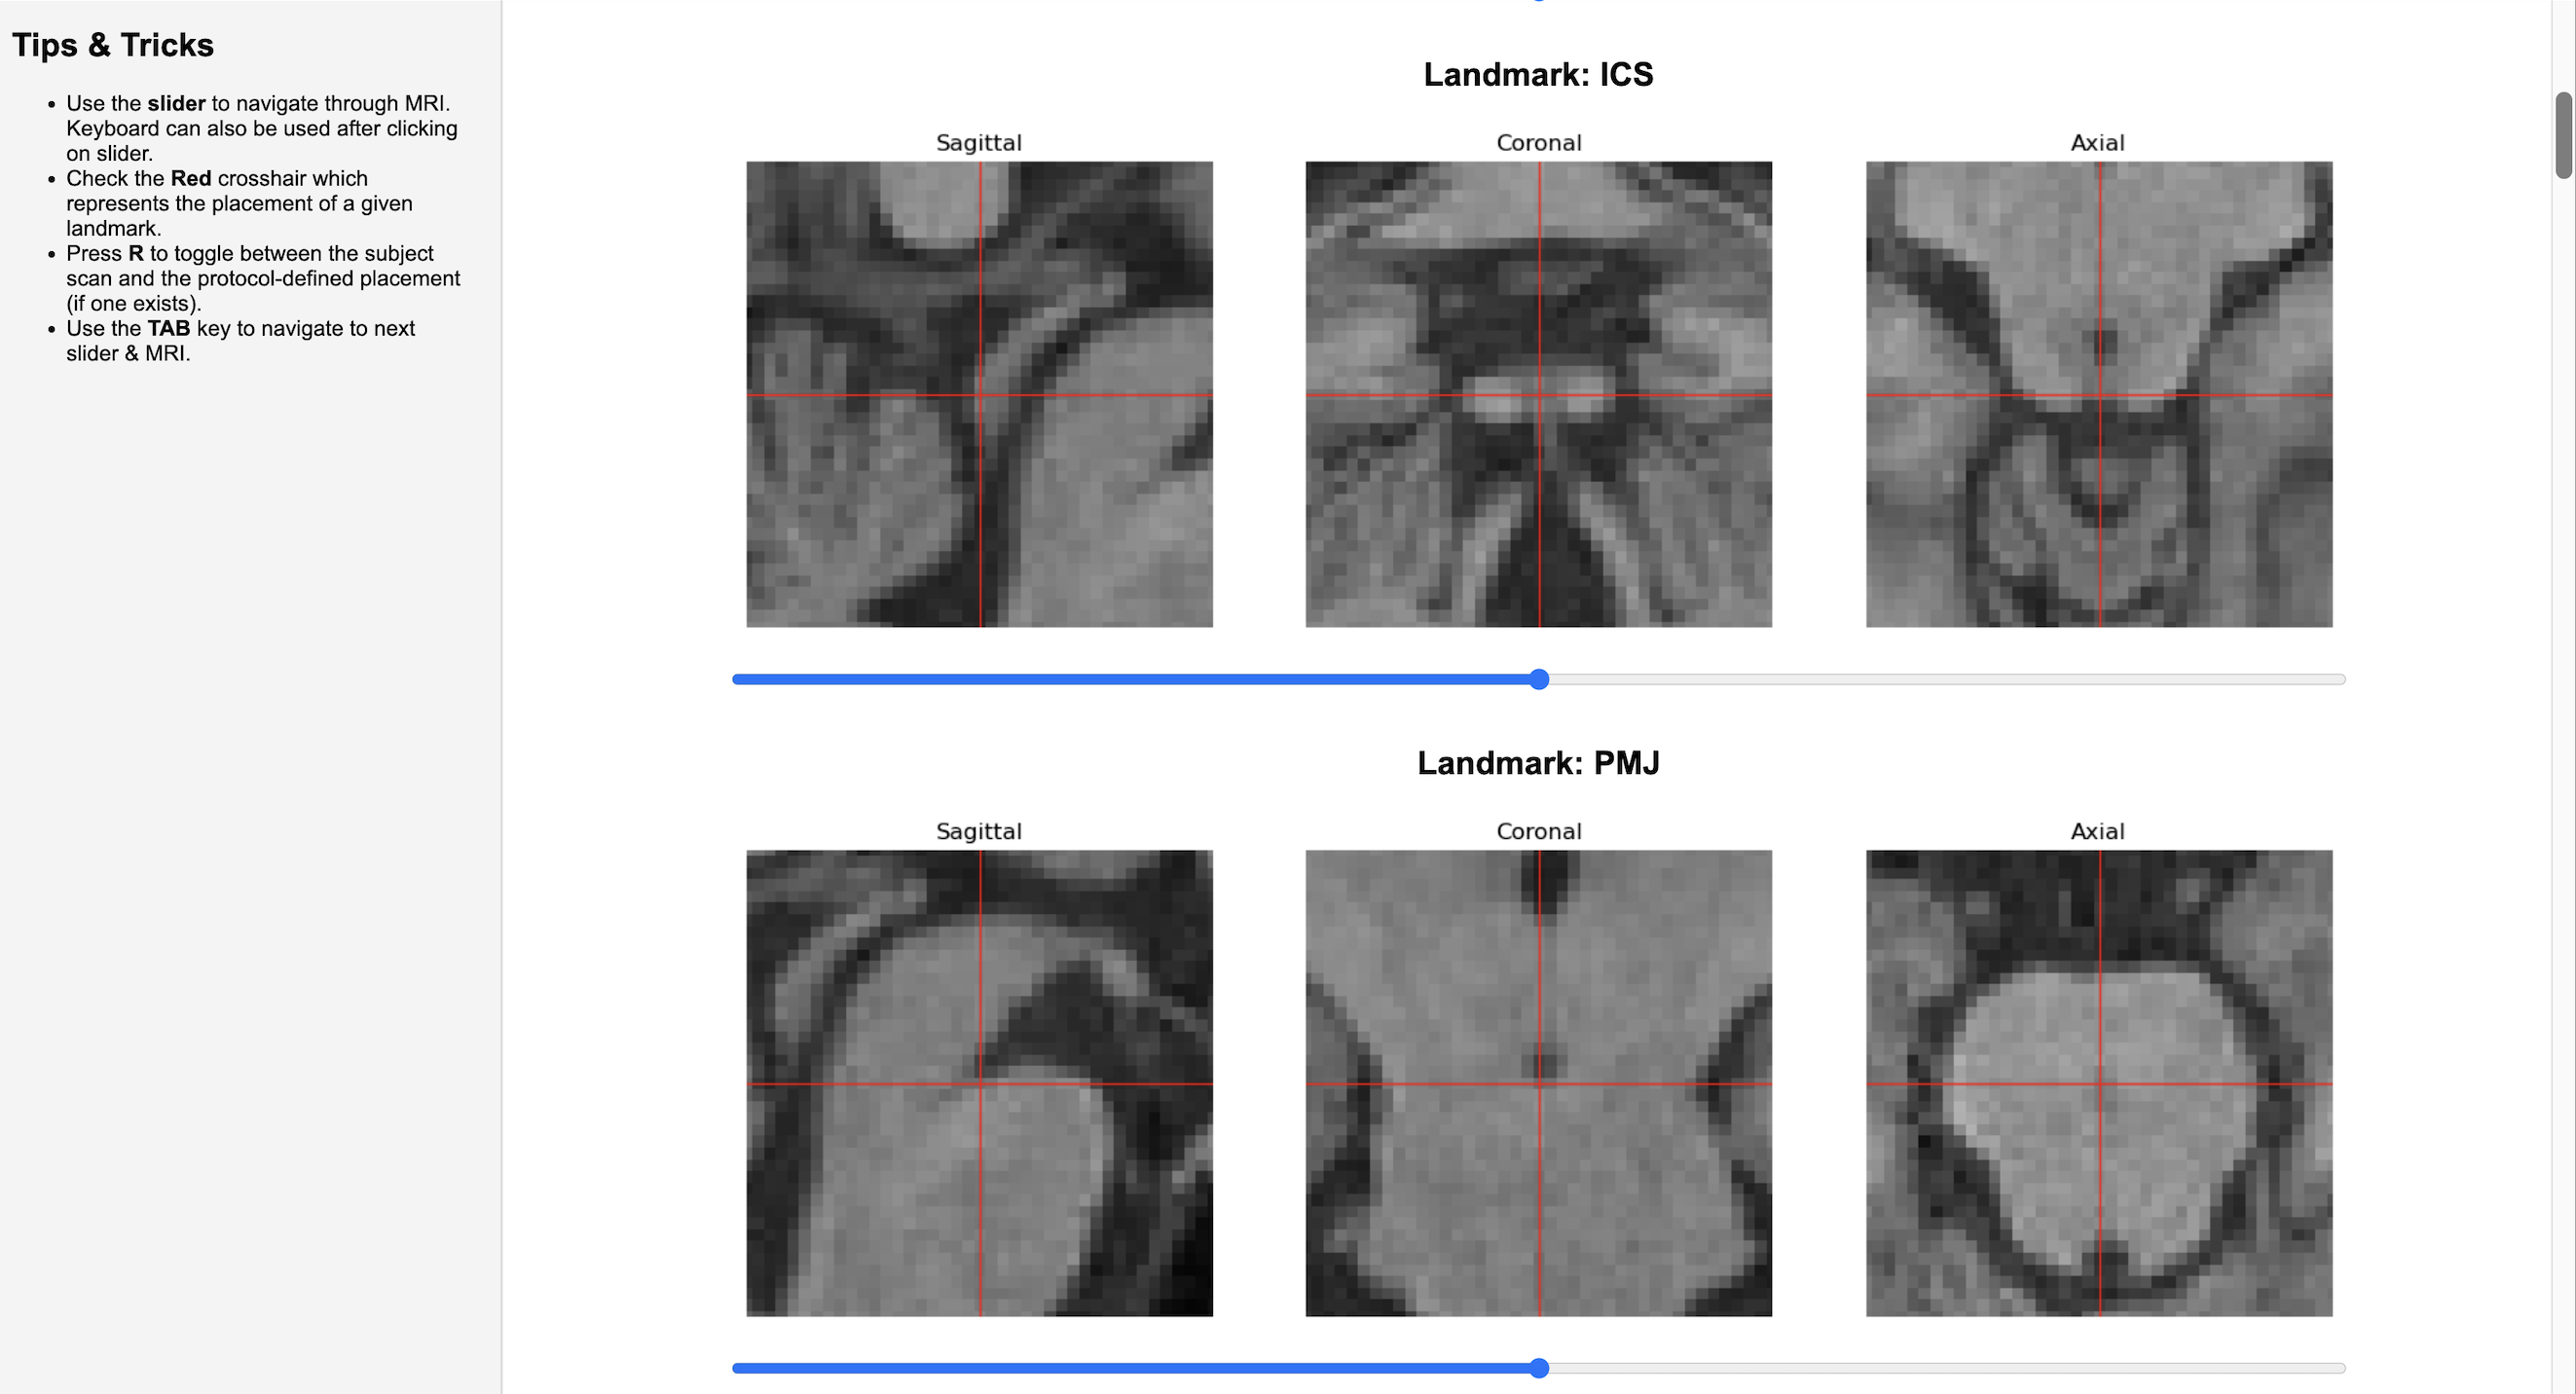
\includegraphics[width=0.95\linewidth]{figs/figuresupQC.png}
    \caption{Quality control visualization for anatomical landmark placement. Crosshairs indicate the annotated location of an example fiducial (the infracollicular sulcus [ICS]) in sagittal, coronal, and axial MRI views. Reviewers can toggle between the subject scan and the protocol-defined (template) annotation using the R key while navigating select slices in MRI volume using arrowkeys or slider.}
    \label{fig:figuresupQC}
\end{figure}

\section{Title 3}\label{app:Chapter4}

Another subsection

\begin{theorem}
Theorem here.
\end{theorem}

\begin{proof}
    Proof here.
\end{proof}